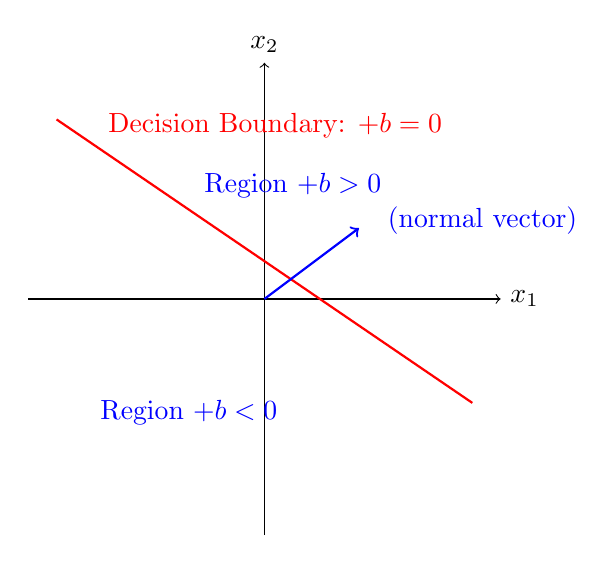
\begin{tikzpicture}[scale=1.2]
  \draw[->] (-2.5,0)--(2.5,0) node[right] {$x_1$};
  \draw[->] (0,-2.5)--(0,2.5) node[above] {$x_2$};
  \draw[thick, red] (-2.2, 1.9) -- (2.2, -1.1) node[pos=0.1, above right] {Decision Boundary: $\w\T\x + b = 0$};
  \draw[blue, thick, ->] (0,0) -- (1, 0.75) node[pos=1.1, right] {$\w$ (normal vector)};
  \node[blue] at (0.3, 1.2) {Region $\w\T\x+b > 0$};
  \node[blue] at (-0.8, -1.2) {Region $\w\T\x+b < 0$};
\end{tikzpicture}
